\chapter{Implementation}
The implemention of the application can roughly be divided into two parts: A server, being the layer between the user and the database, and a client presenting the data to the user. This chapter will describe the requirements for each part, the technical challenges of the project and how they were met.


\section{Choice of platform}
We decided to create a web based solution instead of a desktop application, mostly based on the nature of the project but also on our own interests. The web based solution does not require a client to be installed on the users system, which makes it instantly accessible. The webbased solution also makes the program available on any device with an internet connection; from a laptop, a smartphone or a dedicated monitor at ITU.\\

This is of course a tradeoff, as we have much more experience with developing desktop applications, which would probably be much faster and cause fewer errors to debug. However, we do think it was a natural choice to put the application on the internet, because of the large number of people who will use it everyday.

\section{Language}
Since we mainly focus on the UI, we wanted to use a framework for the development process, giving us some functionality "out of the box". This would reduce the time spent on the technial implementation, and give us more time to focus on the UI.\\
We have chosen to use \emph{Scala}\cite{scala} as the implementation language; a multi-paradigm language running on the JVM. Scala is a superset of java, featuring some functional programming constructs, like pattern matching and immutable types. While it is possible to use the java libraries, Scala provides many immutable alternatives to make concurrent programming easier. \\

A large motivation for choosing Scala, was the rich functionality provided by the Scala based web framework \emph{Lift} \cite{lift}. Lift is designed as a framework for developing web applications, with a high focus on security and performance. Lift provides us with the following functionality relevant to our project:

\begin{itemize}
	\item \textbf{Sitemap}\\
	A sitemap is used to represent the structure of a website. Each page in the structure can be specified to require a certain level of authorization to be accessible. \\
	\item \textbf{Sessions}\\
	Lift support handling of multiple users with sessions. A session is a cookie, with some information about the user associated with it.\\
	\item \textbf{Xml bindings}\\
	Lift uses xml as reference points for dynamic code injection. The static parts of the application are built using normal HTML. XML are used as placeholders, or bindings, for the data that are supposed to change during a session. This makes it possible to completely seperate the development of the presentation layer (the client), and the data layer (the server).
\end{itemize}

Lift is thus giving us a lot of the functionality we need to make our application work, but it also poses a large challenge, as Lift requires decent experience with Scala, which we do not yet have.

\section{Development environment}
\label{sec:development_environment}
During development, we have used a tool called Simple Build Tool(SBT)\cite{sbt} to compile and test our application. SBT comes with a local web server (called Jetty), and a Lift project template, seperating the client and server. Appendix \ref{app:lift_structure} describes the basic structure of such a project.\\
SBT support automatic compiling, so when a file included in the project is changed, Jetty will automatically compile the changed file(s) and restart the webserver. Appendix \ref{sec:setup_and_use} contains a setup and user manual for the application.

\section{Technical requirements}
\label{sec:tech_req}
This section describes the technical requirements for the server and the client. General requirements have been described in section \ref{subsec:functional_requirements}, and the actual implementation will be discussed in section \ref{xxxx}.

\subsection{Server}
\label{sub:req_server}
\begin{itemize}
	\item \textbf{General authorization}\\
	The server should not allow access to the system unless the user is logged in. The sitemap functionality in Lift should be used to request authorization and present the appropriate pages.
	\item \textbf{User levels}\\
	In our system, we need two different user roles; one for staff members which should have access to the semester planning application(\emph{super users}), and one for all other users (\emph{basic users}). Specific user roles are assigned an integer indicating the users \emph{level}. Super users are level 2, while basic users are level 1. The server should use the sitemap to only present the semester planning to super users, thus users with a level of 2. 
	\item \textbf{Support of multiple users}\\
	Lift Sessions should be used to distinguish users from each other. The Session associated with a user is not a placeholder for the actual user \emph{object}, but merely a unique identifier. The Session cookie should only contain the unique ID of the user, fetched from the database.
\end{itemize}

\subsection{Client}
\label{sub:req_client}
\begin{itemize}
	\item \textbf{Clickable map with server callback}\\
	The client should present a clickable map of the rooms at ITU. When the user selects a room, the view should change and let the user book the selected room for the current day. This requires that the client sends data to the server, which is usually done within a <form> element using a submit button. However, as we are dealing with a clickable image, this is not an option. Lift does not support interactions with images, but does support callbacks from javascript functions. We can thus use a html clickable map\cite{html_map}, and attach a javascript callback through Lift, enabling us to call a function when the user selects a room.
	\item \textbf{Interactive Calendar}\\
	The users should be able to select a different day than the current, giving them the option to book a room in advance. JQueryui\cite{jqueryui} offers a datepicker widget\cite{jqueryui_date}, which supports this functionality.
	\item \textbf{Custom time and day picker}\\
	Because our day and time picker \ref{chap2_req:xx} is a custom made widget and very application specific, it has to be made from scratch. Since Lift support callbacks through javascript, it's possible to create such a widget by using this functionality together with simple html attributes as date and time identifiers.
	\item \textbf{XML Exporter}\\
	It should be possible to export the data created during semester planning. Since the data will be used in multiple ways (for printing, digital archiving, etc.) the output should be in XML for maximum application support.\\ 
The exporter has to be manually created, e.g. by using a Java XML generator.
\end{itemize}

\section{Database design}
\label{sec:database_design}
From the requirements in section \ref{sec:requirements} and the technical requirements above, we derived the database design seen in figure \ref{fig:db_design}. While parts of the design are trivial, here follows the ideas behind some of the more non trivial elements.

\begin{figure}[htb]
\begin{center}
\leavevmode
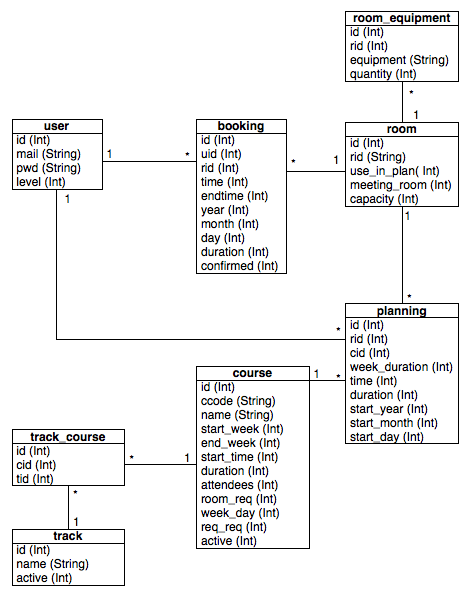
\includegraphics[width=0.6\textwidth]{images/db-design.png}
\end{center}
\caption{Database design}
\label{fig:db_design}
\end{figure}

\subsection{Course and planning table}
\label{sub:course_planning_table}
The course tabel contains information about a specific course. It should be possible to create a course without immediately adding it to the semester planning, which is why the two tables seem to contain some of the same data. The \emph{room\_req} field is a \emph{room request} field. We learned from section \ref{xx} that teachers often have specific room requests, which this field reflects. This might be a wish, or an actual request which should be respected by the application, if e.g. a course requires equipment only available in one room. In that case, the \emph{req\_req} field is set to 1, indicating that this is a constraint and not a wish. 

\subsection{Day and time modelling}
\label{sub:day_and_time_modelling}
We have chosen not to use the built in date field type in MySQL, because we use javascript to exchange data between the client and the server. Javascript does not understand this data type by default, and while it might be possible to write a function that creates an object representing the same type, we will still have to deal with string splitting and concatination. This is very inefficient and takes up more space compared to using simple integers.\\
We have thus used integers to represent all kinds of date and time data. An example is the \emph{booking} table, which contains information about a specific booking. \emph{time} and \emph{endtime} represents the start time and end time of the booking respectively, by the number of minutes after midnight. If a booking starts 10.30 in the morning, the start time field will thus be 630. This way of representing the time has a couple of advantages:

\begin{itemize}
	\item Simple calculations can be used to find the duration of a booking, and the actual time the fields represent. We do not need to work with strings, which makes the code clearner and more efficient.
	\item For the same reason, user validation is quick and easy to perform.
	\item We can still execute specific date and time sql queries by using basic relationel operators, which makes it more efficient to e.g. lookup bookings after a specific time.
\end{itemize}

\section{Concurrent room selection}
\label{sub:challenges_concurrent_rooms}
While we expect a lot of users to actively using our application at the same time, the problem with concurrent room selections has to be adressed. While the actual implementation has been left out because of our focus for the project, we have had a lot of considerations about how this can be solved.\\

\subsubsection*{Scenario and possible solutions}
These solutions are based on the simple scenario where users \textbf{X} and \textbf{Y} are searching for rooms at the same time. They could obviously be extrapolated to cases where even more users are interacting. We assume that \textbf{X} was the first user to click the search button. Online users should be tracked, to make the logging possible.
\subsubsection*{Hide bookings from certain users}
\begin{tabular}{|p{6cm}|p{6cm}|}
\hline 
	\multicolumn{2}{|p{12cm}|}{Make all rooms that fits \textbf{X}, unavailable for \textbf{Y} while \textbf{X} is deciding on which room to use.} \\ \hline \hline
	\multicolumn{1}{|c|}{\textbf{Pros}} & \multicolumn{1}{c|}{\textbf{Cons}} \\ \hline
	Easy to implement & If all rooms fit the search of \textbf{X}, no rooms will be available for \textbf{Y}. If there are 10 rooms in total, and 10 users search for 10 random rooms, no rooms will ever be available for the next user. \\
	\hline
\end{tabular}
\\
\subsubsection*{Dynamic refresh}
\begin{tabular}{|p{6cm}|p{6cm}|}
\hline
	\multicolumn{2}{|p{12cm}|}{The screen which shows available rooms for user \textbf{Y} should update when user \textbf{X} selects a room for booking.} \\ \hline \hline
	\multicolumn{1}{|c|}{\textbf{Pros}} & \multicolumn{1}{c|}{\textbf{Cons}} \\ \hline
	High usability and responsiveness & Increased number of requests to the server. \\ \hline
	More flexible; allows several users to have many choices at once. & If user \textbf{X} changes his mind during a booking, user \textbf{Y} misses a valid opportunity to book the room.\\
	\hline
	\multicolumn{2}{|p{12cm}|}{Ultimately, this solution is a tradeoff between the probability of concurrent selections occuring and server-request rate. If the server is set to refresh each second, this might reduce the probability of errors, but the server might not scale very well.} \\
	\hline
\end{tabular}
\subsubsection*{User awareness}
\begin{tabular}{|p{6cm}|p{6cm}|}
\hline
	\multicolumn{2}{|p{12cm}|}{Information about whether or not other users are looking at the same room will be presented for the user, to make him/her aware that other people might be interested in the room. } \\ \hline \hline
	\multicolumn{1}{|c|}{\textbf{Pros}} & \multicolumn{1}{c|}{\textbf{Cons}} \\ \hline
	It does not come as a sudden surprise if the room is booked before them. & Increased number of requests to the server. \\ \hline
	\multicolumn{2}{|p{12cm}|}{Basically this is not a different solution than \textbf{dynamic refresh}, but just a way of minimizing the server requests, making it perform better, but increases the probability of concurrent selections.} \\
	\hline
\end{tabular}

Of all these solutions, the most effective would be \textbf{dynamic refresh}. This is however also generating the most server requests, but since the number of seconds between each refresh can be varied, this seems like a flexible solution as well. It could be made even better, by making each client sending a signal to the server when a booking was made, so the server could notify the clients.\\

\todo{Write an implementation section for both the client and server. Mention the use of photoshop!}
\section{Actual implementation}
\label{sec:actual_implementation}

\subsection{User authorization}
User authorization has been implemented using the built in Sitemap feature of Lift. In a Boot file, used to initialize the program, a sitemap object is created:

\begin{verbatim}
    val siteMap = SiteMap(
        Menu("Index") / "index"	>> AuthRequired >> Hidden,
        Menu("Advanced") / "advanced" >> Hidden,
        Menu("RoomBooking") / "room-booking" >> AuthRequired >> Hidden,
        Menu("Login") / "login" >> LoginAuth >> Hidden,
        Menu("Your Reservations") / "reservations" >> AuthRequired,
        Menu("Logout") / "logout" >> EarlyResponse(() => {
            Session.loggedIn.apply(0)
            Full(RedirectResponse("login"))
        })
    )
    // Tell Lift to use our sitemap
    LiftRules.setSiteMap(siteMap)
\end{verbatim}

Each line represents one page, which is added to the static menu simply by using its constructor. The name after the slash is the actual name of the html page. A page can be assigned several functions which should be called before each page is evaluated and shown. In our sitemap, all pages should call the \emph{AuthRequired} function, which redirects the user to the login page if not logged in. Several pages calls the \emph{Hidden} function, which is a built in function in Lift. Hidden pages are not shown in the menu, and cannot be accessed directly. \\
The logout menu item uses an anonymous inner function, to sign out the user, by setting the session cookie to 0 (see section \ref{sub:sessions}), and redirecting to the login screen.\\

\subsection{User sessions}
\label{sub:sessions}
Handling of multiple users in Lift is done by using the built in \emph{SessionVar} class:

\begin{verbatim}
    object Session{
        object loggedIn extends SessionVar[Int](0)
        object uid extends SessionVar[Int](-1)
        object currentRoom extends SessionVar[String]("-1")
    }
\end{verbatim}

While our \emph{Session} object is static, a cookie for each SessionVar is stored on the users computer when the object is created, thus making it possible for the users to share the global Session object, while still having individual data stored in the SessionVar object. \\
As an example, take the uid object. This extends a SessionVar of type Int, with a default value of -1. When the user signs in, this value is changed from the default value to the specific id of the user, fetched from the database.\\

Setting and retrieving the values can be done in constant time:
\begin{verbatim}
	// In another class, do something with the user id
	room.book(Session.uid.is)
	
	// ... Change it, e.g. when the user signs out
	Session.uid.apply(-1)
\end{verbatim}
This is a convient way of always having access to the unique id of the user.

\subsection{Quickbooking}
\label{sub:quickbooking}
When the user click the \emph{Quick Booking} button on the frontpage (see ref \ref{xx}), the application searches the database for an optimal room(see section \ref{scope}).\\

JQuery is used to attach a click-listener to the button:

\begin{verbatim}
jQuery('#quickfind').click(function(){
    liftAjax.lift_ajaxHandler('""" + funcName2 + """='+uid, null, null, null);
});
\end{verbatim}

\emph{funcName2} Queries the database for an available room, and returns the room id if any is found:

\begin{verbatim}
    val func2 = () => {
        var roomid = Database.findRoomNow
        if(roomid != -1){
            var booking = Database.bookRoom(rid = roomid)
            ...
        }
        else{
           // No rooms
           ...
        }
    }
\end{verbatim}

The \emph{bookRoom} function of the \emph{Database} object only takes a single parameter. Other options are automatically assigned by predefined method signatures:

\begin{verbatim}
def bookRoom(uid : Int = Session.uid.is, rid : Int, 
             from : Int = now, to: Int = now + 240){ ... }
\end{verbatim}

Here, the user id (uid) is retrieved from the \emph{Session} object, the beginning time of the booking is set to the current time, and the booking is by default set to last 4 hours. \\
The function books the room, and notifies the user.\\

If the user for some reason changes his mind and wants to cancel his booking, the cancel button can be used. This will delete the booking that was just created. \\
It might seem strange that we first book the room, and then cancels it, instead of just booking the room when the user accepts it. However, by booking the room immediately, we avoid concurrency issues which could occur if user \textbf{Y} books the same room as user \textbf{X} is about to accept.

\subsection{Simple Booking}
The Simple Booking time selector function had to be implemented from scratch, as it was highly application specific. We wanted to make a function that allowed the user to select a time range, on a specific day of the week. (See section \ref{xx} for screenshots of this functionality). \\
We desided to only use Javascript for this, by including all relevant information in the html tags, and only use Lift to call a function to book the room in the selected time span. Each day is divided into blocks from 7 in the morning to 21 in the evening. It is possible to select even and half hour blocks:

\begin{verbatim}
    for(var j = 7; j < 21; j++){
        t = j * 60;
        t30 = t + 30;
        html = html + '<div class="timeBlock block'+t+'"></div>';
        if(j != 20) {
            html = html + '<div class="timeBlock block'+t30+'"></div>';	
        }
    }
\end{verbatim}

Block420 is thus the block representing 420 minutes after midnight = 7 in the morning. JQuery is used to store the time values when a user clicks on a timeblock. JQuery can react on all elements with the class timeblock, and use the \emph{this} selector to reach just the element the user selected:

\begin{verbatim}
    $("#theGrid li").not(".topLabel").find(".timeBlock").click(function(){
        beginClick = (!beginClick);
        var timeSelector = (($(this).attr('class')).split(" "))[1];
        var timeLabel = $("#theGrid ul li.topLabel").find("."+timeSelector);
    });
\end{verbatim}

The \emph{timeLabel} variable are set to the node in the header which has the same \emph{timeSelector} class as the block the user selected. The actual time is shown in human readable form in the inner html of the header, making it easy to retrieve the actual time the user selected through this node, by calling the \emph{html()} function of the \emph{timeLabel} variable.